\section*{Überblick}

\paragraph{Nervensystem --- Überblick}
\begin{itemize}
  \item Unterscheidung nach Lage
  \item \textbf{Zentrales Nervensystem} (ZNS): Gehirn und Rückenmark
  \item \textbf{Peripheres Nervensystem} (PNS): Außerhalb von Gehirn und Rückenmark
  \item \textbf{Autonomes Nervensystem} (ANS): Steuerung lebenswichtiger Funktionen
\end{itemize}

\paragraph{Autonomes Nervensystem --- Unterteilung}
\begin{itemize}
  \item \textbf{Sympathisches Nervensystem} (\emph{fight or flight}): Bei Stressreizen \( \to \) Notfallfunktionen des Organismus werden aktiviert:
  \begin{itemize}
    \item Steigerung Puls + Blutdruck + Blutglukosespiegel (mehr Energie)
    \item Steigerung Aufmerksamkeitslevel + Schweißproduktion
    \item Vergrößerung Pupillen
    \item Erhöhung Muskeltonus (= Grundspannung der Muskel)
  \end{itemize}
  \item \textbf{Parasympathisches Nervensystem} (\emph{rest and digest}): Stoffwechsel + Aufbau Körperreserven bei Erholung:
  \begin{itemize}
    \item Reduktion Herz-Pumpleistung
    \item Steigerung Darmaktivität
  \end{itemize}
\end{itemize}

\paragraph{Dermatom + Spinalnerv}
\begin{itemize}
  \item \textbf{Spinalnerv}: Nerv, der zu einer bestimmten Seite und einem bestimmten Rückenmarksegment gehört (zw. 2 Wirbeln treten jeweils 2 Spinalnerven aus Wirbelkanal)
  \item \textbf{Dermatom}: Hautbereich, der von den sensiblen Fasern einer Spinalnervenwurzel autonom versorgt wird.
\end{itemize}
\begin{figure}[H]
  \centering
  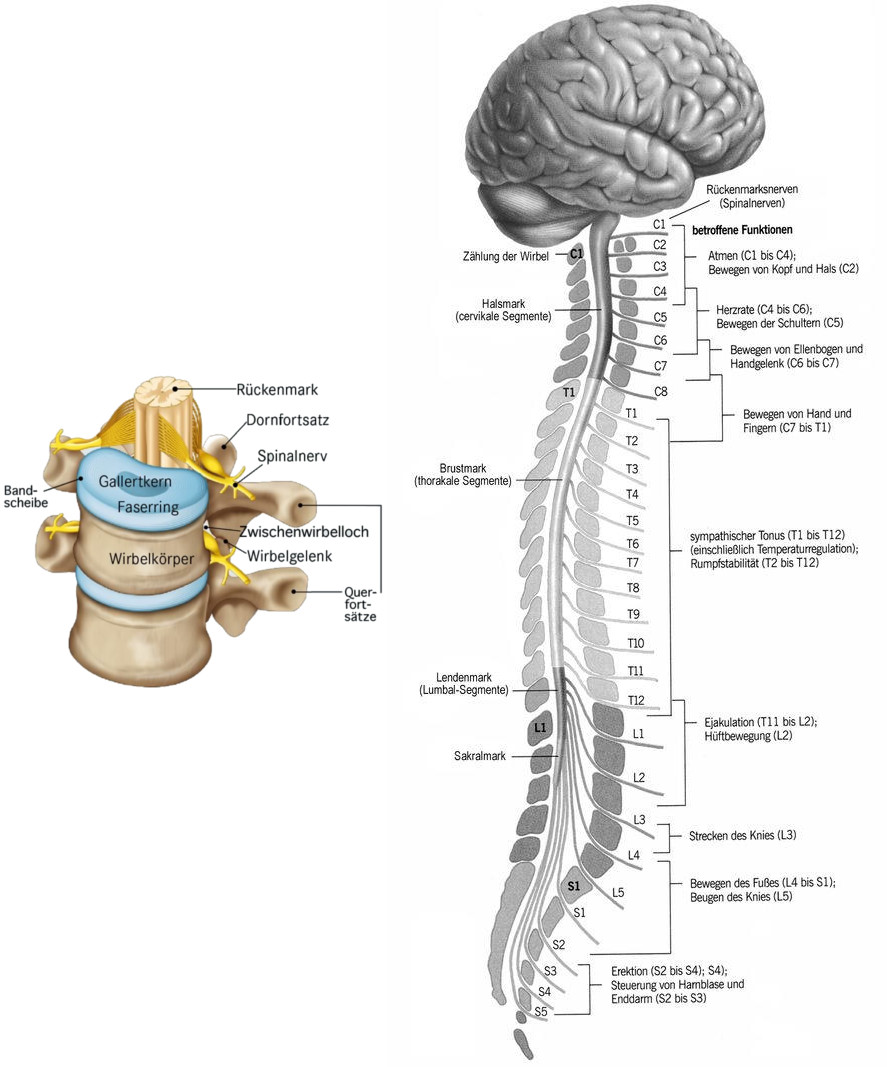
\includegraphics[width=\linewidth]{assets/img/rueckenmark.jpg}
\end{figure}

\paragraph{Hirnnerven}
\begin{itemize}
  \item Besondere Paar-Nerven mit Ursprung im Hirn (statt Rückenmark)
  \item Nummerierung: römisch von oben nach unten (je nach Austrittsstelle)
\end{itemize}

\paragraph{Nerven}
\begin{itemize}
  \item Kommunikationssystem des Körpers
  \item Geben Impulse zwischen ZNS und Körperbereichen weiter
  \item Bestehen aus vielen Neuronen
  \item Ernährung + Sauerstoffversorgung durch Blutgefäße
  \item \textbf{Aufbau}:
  \begin{itemize}
    \item Nervenfaserbündel, umgeben von Bindegewebshülle
    \item Alle Bündel umgeben von weiterer Bindegewebshülle (hält alle zusammen)
  \end{itemize}
\end{itemize}